%%
%% Dit is een onderdeel van abi-instructie.tex
%%
\section{Projectstappen op hoofdlijnen}

De activiteiten binnen ABI kunnen in een viertal fasen opgedeeld worden.
De eerste twee fasen hebben te maken met de voorbereiding van het voor de
opdrachtgever uit te voeren project. De fase 3 betreft de uitvoering van dit
project en de fase 4 de afronding.

\begin{figure}[!ht]
    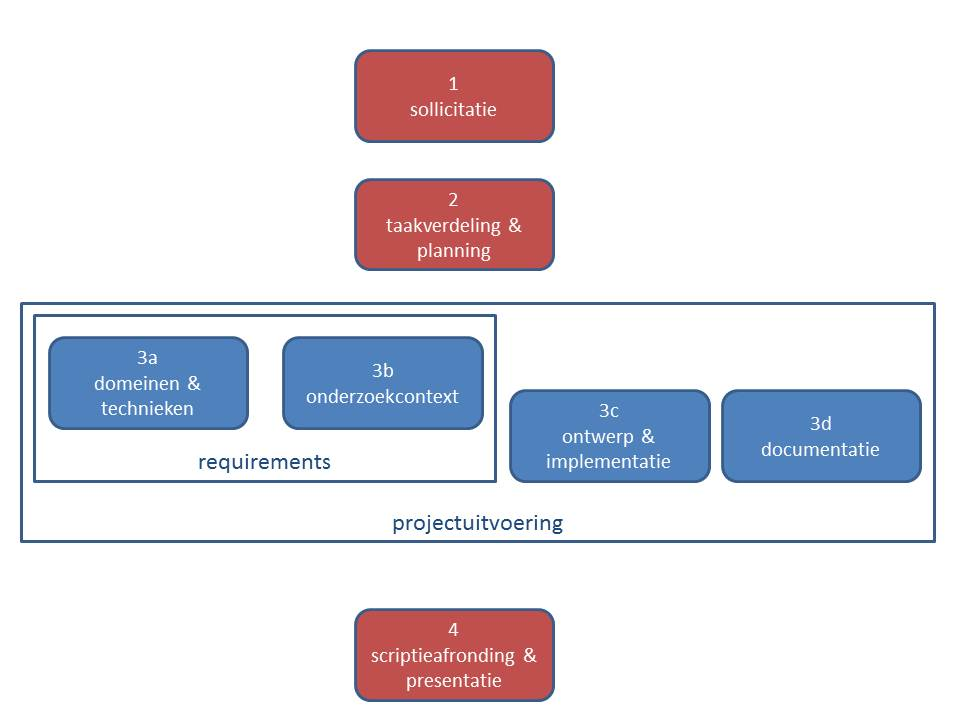
\includegraphics[width=\textwidth]{./overview.jpg}
    \label{fig:overview}
    \caption{De globale planning: overview}
\end{figure}

Voor elk van de fase 2 en 4 en de deelfasen 3a t/m 3d staat een nominale
doorlooptijd. Elk van deze fasen wordt afgesloten met een mijlpaaldocument
dat kwalitatief beoordeeld wordt door de begeleider. Alleen de fase 3a
wordt afgesloten met een individueel mijlpraaldocument,  de overige mijlpaalproducten
zijn groepsproducten.

Het eindcijfer wordt bepaald door de examinator, rekening houdend met de
kwalitatieve beoordelingen van de begeleider.

Gedurende het gehele proces vindt er tenminste een (virtueel) maandelijks
overleg plaats tussen het gehele team en de begeleider. Input voor dit
overleg zijn de individuele maandrapportages en de eventuele mijlpaaldocumenten
die u in de afgelopen maand opgeleverd heeft.

Van elk mijlpaaldocument worden slechts 2 versies door de begeleider
beoordeeld. Op een conceptversie ontvangt u feedback met
verbetervoorstellen en de tweede versie wordt beoordeeld.

\begin{figure}[!ht]
    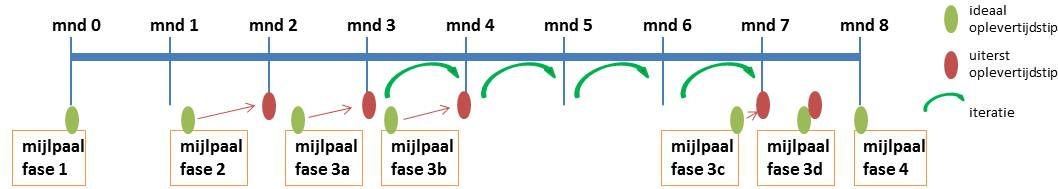
\includegraphics[width=\textwidth]{./globale-tijdsplanning.jpg}
    \label{fig:globale-planning}
    \caption{De globale planning: volgorde van mijlpaalproducten}
\end{figure}

Afbeelding \ref{fig:globale-planning} geeft een indicatie omtrent de
opleveringtijdstippen van de verschillende mijlpaalproducten na de
start van het ABI-project. Groene bolletjes geven de ideale
oplevertijd weer en rode bolletjes de uiterste oplevering
per mijlpaalproduct.

Ook zijn de mogelijke iteraties getoond maar het aantal
iteraties en de duur van een iteratie bepaalt u als team
in overleg met de opdrachtgever.

\subsection{Voorbeeldplanning}
Een ``ideale'' planning bij een start in september dan wel februari
ziet er als volgt uit.

Deze planning geeft een beeld van de verhouding tussen de inspanningen
in de verschillende fasen.Uiteraard maakt u als team in fase 2 een eigen
planning en er kunnen allerlei goede redenen zijn om af te wijken van
de ideale planning. Zeker de activiteit 3c vraagt ook om een nadere
uitsplitsing; bv. in de vorm van sprints van 3-4 weken. Ook is het
raadzaam om in fase 2 al na te denken over een mogelijke einddatum
van het project waar als team naartoe gewerkt wordt zodat de verwachtingen
bij alle betrokkenen helder zijn.
De midterm bijeenkomsten zijn medio november en medio april.

%%
%% De voorbeeld planning runs op het web kloppen niet, zijn inconsistent.
%% Met name de voorbeeld duren en start en eindtijd van de 3b, 3c en 3d
%% subfasen zijn vreemd. De volgorde klopt ook niet. Enigzins aangepast, maar nog niet correct.
%%
%%

\begin{framed}
    \begin{center}
	\begin{tabular}{lllr}
	    \textbf{fase} & \textbf{doorlooptijd} & \textbf{voorbeeld} & \textbf{netto}\\
	    fase 2        & 1.5  & medio sept - eind okt & 20\\
	    fase 3a       & 2    & eind sept - eind nov & 50\\
	    fase 3b       & 2    & eind nov - eind dec & 30\\
	    fase 3c       & 5    & eind nov - eind apr & 230\\
	    fase 3d       & 2    & eind mrt - eind apr & 50\\
	    fase 4        & 1.5  & eind mrt - medio mei & 20\\
	\end{tabular}
    \end{center}
    \captionof{table}{Run vanaf september}
 \label{fig:sept-run}
\end{framed}

\begin{framed}
    \begin{center}
	\begin{tabular}{lllr}
	    \textbf{fase} & \textbf{doorlooptijd} & \textbf{voorbeeld} & \textbf{netto}\\
	    fase 2        & 1.5  & medio febr - eind mrt & 20\\
	    fase 3a       & 2    & eind febr - eind apr & 50\\
	    fase 3b       & 2    & eind mrt - eind mei & 30\\
	    fase 3c       & 5    & eind apr - eind sept & 230\\
	    fase 3d       & 2    & eind mrt - eind sept & 50\\
	    fase 4        & 1.5  & eind sept - medio okt & 20\\
	\end{tabular}
    \end{center}
    \captionof{table}{Run vanaf februari}
 \label{fig:febr-run}
\end{framed}
